\documentclass{../local}
\begin{document}
\section{REXOS Overall Architecture}
% How we changed the architecture, and why we made which decisions
\begin{figure}[h!]
\flushleft
	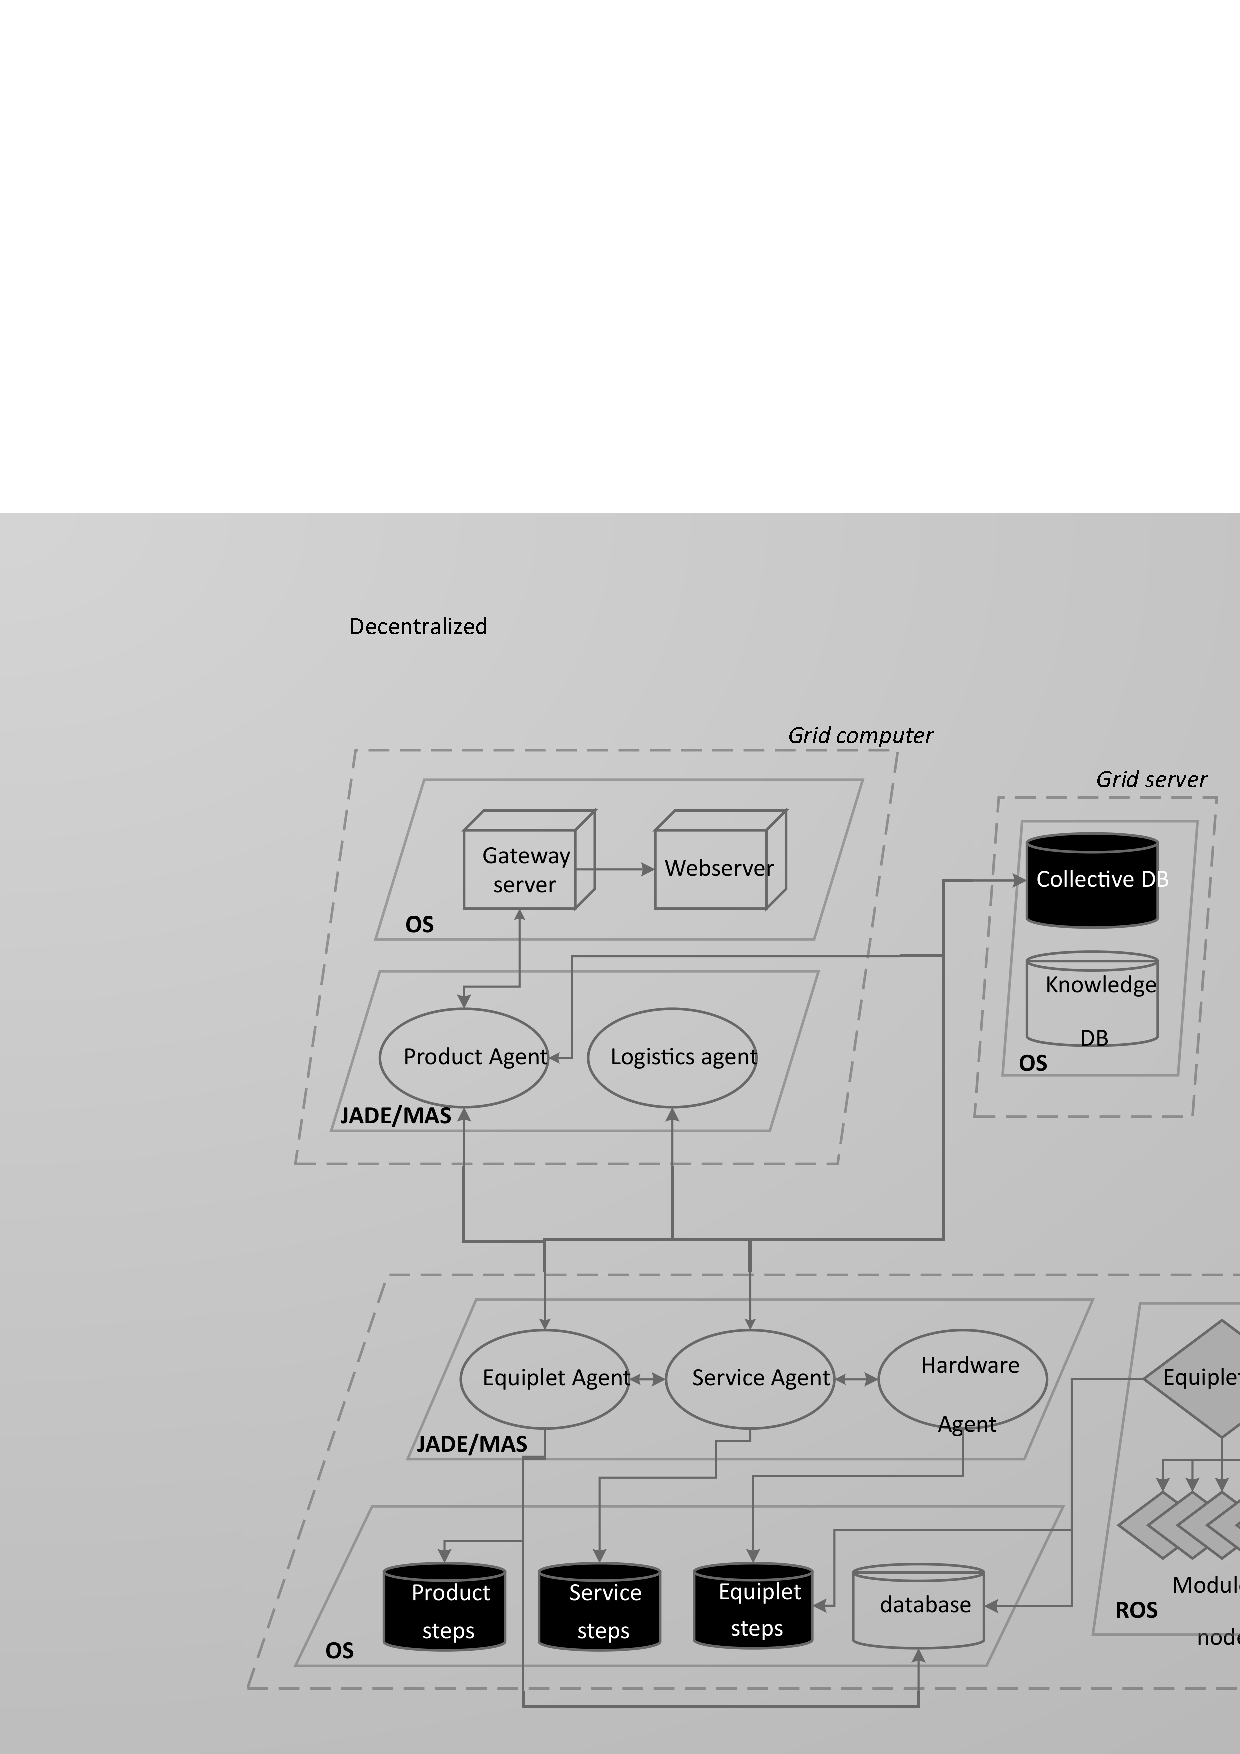
\includegraphics[trim= 9cm 0cm 9cm 0cm, clip=true, width=1.1\linewidth]{../images/Decentralized_REXOS.png}
	%we might want to increase the text on this image..%
	\caption{System overview}
\end{figure}


\subsection{Initial situation}
An overview of the system is given in image 2
\textbf{--INSERT system overview image here ---}

\subsubsection{MAS}
%Tell smth about implementation of the curr MAS system, what purpose it serves, and how its implemented.%
The MAS\footnote{Multi agent system. See abbreviations for more detail.} was designed to be the intelligent and cognitive side of the the REXOS platform. It incorperates virtual autonomous entities known as agents and is implemented in JADE \textbf{ref2section}. As shown in figure \textbf{ref to system overview} there are currently 5 agents. 

\begin{description}
  \item[Product agent] \hfill \\
		The product agents is a representation of the product. It is responsible for scheduling itself with the equiplets it need for finishing the product it represents.
  \item[Equiplet agent] \hfill \\
  		The equiplet agent is responsible for all communication with the product agent. It handles dealing with its own schedule aswell.
  \item[Service agent] \hfill \\
  		The service agent handles all service level translations. 
  \item[Hardware agent] \hfill \\
  		The hardware agent is responsible for 'controlling' the hardware. It also handles module step translations.
  \item[Logistics agent] \hfill \\
  		The logistics are handles all logistics within a grid. Its responsibilities include providing information about parts.
\end{description}

The MAS also provides a product abstraction. This means that a product 

The current implementation of the MAS is lacking both capability and structure. Previous groups of students have worked on the project and set up the basic version of the MAS. 

\subsubsection{Communication}
%smth about the current communication situation%


\subsubsection{ROS}
%Tell smth about implementation of the curr ROS system, what purpose it serves, and how its implemented.%
The current ROS side of the system represents all the hardware in code. All ROS actions are non-autonomous and driven by the intelligent side of REXOS. This means that all MAS-Agents take smart and cognitive decisions and ROS executes these. 
\\
The main focus of this research project was to improve the REXOS platform as it exists today. As described in section \ref{sec:InitialSituation} the architecture was buggy, and not properly implemented. Besides implementing and / or researching a better architecture, a need for new kind of implementation was present as well.

\subsection{Planning - TODO}
The normal planning algorithm used in the simulator is taken from \emph{L. van Moergestel’s paper ‘Multiagent-based agile manufacturing: from user requirements to product.} \textbf{- INSERT QUOTE HERE - } and the batch scheduling algorithm is described below. Scheduling is done by the product agent, which represents a product.
The product consists of steps, which are specific tasks defined by a set of parameters. Think of screwing, glueing or welding. All the equiplets in a grid can perform a certain set of these tasks. The ability to perform such a task is called a capability.  Each equiplet only has a limited set of these capabilities.

In the simulation a grid consisting of equiplets is defined. Each equiplet has its own set of capabilities. Now consider a product with an n amount of product steps($\phi$):\\

$< \phi_1, \phi_2, ... \phi_n >$\\

Once the product (agent) spawns, it will match all possible equiplets to complete all of its steps. Meaning that it compiles a collection containing equiplets combined with the product steps they can perform. That seems like a lot, but the equiplets do not have a large set of capabilities. The resulting collection is:\\

$< E1(\phi_1, \phi_3), E2(\phi_2, \phi_3, \phi_1), E3(\phi_1) >$\\

Once this collection has been compiled,  the product(agent) starts negotiating with the equiplets. It informs with each of the equiplets to evaluate whether or not the step can be performed with the given parameters at the given equiplet.  Once all equiplets have been queried and matched, the actual planning begins.
The first step in the planning consist of reducing the transition time between product steps. First a production matrix is constructed. The rows represent the equiplets while the columns represent the product steps.
goog
\begin{table}[htbp]
\centering
\normalsize
\begin{tabular}{|l|l|l|l|l|l|}
\hline
	& $\phi$1 & $\phi$2 & $\phi$3 & $\phi$4 & $\phi$5 \\
\hline
Equiplet 1 & 1.0 & 0.0 & 1.0 & 1.0 & 1.0 \\
\hline
Equiplet 2 & 0.0 & 1.0 & 0.0 & 0.0 & 0.0 \\
\hline
Equiplet 3 & 0.0 & 0.0 & 0.0 & 0.0 & 1.0 \\
\hline
Equiplet 4 & 1.0 & 0.0 & 1.0 & 1.0 & 0.0 \\
\hline
\end{tabular}
\caption{Initial production matrix}
\end{table}

First off, all equiplets that are capable of performing a step have their value raised to 1.
The next step is to minimize transition. 


To prevent excess transition between equiplets during manufacturing, all equiplets with sequential steps being performed on the same equiplet have their value raised by the length of the sequence -1.  Resulting in the following matrix:

\begin{table}[htbp]
\centering
\normalsize
\begin{tabular}{|l|l|l|l|l|l|}
\hline
	& $\phi$1 & $\phi$2 & $\phi$3 & $\phi$4 & $\phi$5 \\
\hline
Equiplet 1 & 1.0 & 0.0 & 3.0 & 3.0 & 3.0 \\
\hline
Equiplet 2 & 0.0 & 1.0 & 0.0 & 0.0 & 0.0 \\
\hline
Equiplet 3 & 0.0 & 0.0 & 0.0 & 0.0 & 1.0 \\
\hline
Equiplet 4 & 1.0 & 0.0 & 2.0 & 2.0 & 0.0 \\
\hline
\end{tabular}
\caption{Production matrix after transition optimisation}
\end{table}

As is shown in figure (above) E1 is able to perform step 3, 4 \& 5. The corresponding values where increased by 2 ( sequence length is 3, minus 1 ).

Another easy but important optimization is load balancing. All equiplets are responsible for their own schedule which makes calculating the load at any given time feasible.
Consider a product querying a equiplet to calculate its load for scheduling its 57’th step. This step has to be carried out not at release time, but at release time + $\Delta$ ( where $\Delta$ delta is the time the previous 56 steps will take, including travel time. ) meaning that the equiplet has to calculate load over that time ( called a window).

Consider the following 2 schedules:

%\includegraphics[width=.98\linewidth]{}

If the equiplet would calculate load over release time + window length, it would not be a correct calculation. In above image equiplet 1 has a load of 90\% whereas equiplet 2 has a load of 20\%.
In order to favor the equiplets with least load, all numbers in the matrix are multiplied with ( 1 – (load) ).

Applying this to our current production matrix, and a imaginary constant load ( E1 – 60\%, E2 – 20\%, E3 – 40\% and E4 – 10\% ), the matrix will result in:

\begin{table}[htbp]
\centering
\normalsize
\begin{tabular}{|l|l|l|l|l|l|}
\hline
	& $\phi$1 & $\phi$2 & $\phi$3 & $\phi$4 & $\phi$5 \\
\hline
Equiplet 1 & 0.4 & 0.0 & 1.2 & 1.2 & 1.2 \\
\hline
Equiplet 2 & 0.0 & 0.8 & 0.0 & 0.0 & 0.0 \\
\hline
Equiplet 3 & 0.0 & 0.0 & 0.0 & 0.0 & 0.6 \\
\hline
Equiplet 4 & 0.4 & 0.0 & 1.2 & 1.2 & 0.0 \\
\hline
\end{tabular}
\caption{Production matrix after load balancing}
\end{table}

(steps Ø 3,Ø 4 \& Ø 5 on E1 are multiplied by ( 1 – 0.6 ) which results in 3 * 0.4  )
As seen in the figure above, E1 which has a load of 60\% is suddenly not the best option for steps 3 \& anymore. This way, a proper load balance between the equiplets is achieved.

Another important optimization is reducing the travel time between steps. Much like reducing the transition time between steps that can be executed on the same equiplet, this optimization is meant to reduce travel time within the grid. In order to do so, a distance matrix is utilized. This matrix has equiplets in both the rows as columns, and travel times between these as values ( in amount of timeslots required to travel  from 1 to another ):

\begin{table}[htbp]
\centering
\normalsize
\begin{tabular}{|l|l|l|l|l|}
\hline
	& Equiplet 1 & Equiplet 2 & Equiplet 3 & Equiplet 4  \\
\hline
Equiplet 1 & x & 3.0 & 1.0 & 2.0 \\
\hline
Equiplet 2 & 3.0 & x & 6.0 & 3.0 \\
\hline
Equiplet 3 & 1.0 & 6.0 & x & 6.0 \\
\hline
Equiplet 4 & 2.0 & 3.0 & 6.0 & x \\
\hline
\end{tabular}
\caption{Grid distance matrix}
\end{table}

% this bit till the end of the subsection is missing data? %
Now, utilising the production matrix, the product will try and use a path of least resistance algorithm to find the most suitable path within the grid.




Ignoring all 0 values,  the following possible paths are presented:
 

Combined with the weight of the values in the production matrix, a couple of feasible paths are calculated. These parts are then scheduled sequentially. ( taking the best path first ).

\subsection{Scheduling}
After the production plan has been made, the product agent will then schedule its plan at the corresponding equiplets. The schedule of an equiplet has to be easily accessible and easily to manipulate. Also, calculating the load of an equiplet or gaps in the schedule needs to be fast.

\subsubsection{Representation of an equiplet's schedule }
 \textbf{ in paper70 sections 2.1 and 5.6 } it is described that a planning blackboard (BB-planning) represents the schedule of an equiplet. The paper defines that a circular buffer of timeslots is being used for the storage of scheduled product steps. The number of timeslots within this circular buffer is constant. This also means that a product agent cannot schedule steps later than the said constant number of timeslots. 

Using this approach has several disadvantages when used in an agile manufacturing environment. These disadvantages are mainly performance related.

- A circular buffer has limits to its size. For example: given a size of $\phi$ amount of seconds as a timeslot and the buffer size has to be two hours, there has to be $432000 / \phi$ amount of timeslots available in the circular buffer. 

This would also mean that if the $\phi$ amount of seconds has to be in tens of milliseconds, the circular buffer would increase with a factor 100. A timeslot in tens of milliseconds is a valid case since for example modern pick and place robots can move at 200 picks per minute  \footnote{http://www.expo21xx.com/news/new-staubli-tp80-fast-picker-the-next-generation-of-high-speed-pickers/}. The size of the buffer could also increase into several hours since there are for example low cost 3D printers that could take several hours to complete. 

Another requirement of REXOS is that product agents have to be able to schedule a day in the future with a timeslot length of for example 10 milliseconds. This will result in a circular buffer with 8,6 million items for every equiplet. Which is a lot.

For REXOS we took another approach to avoid this issue. We abandoned the idea of using a circular buffer, but we still need to store the schedules of equiplets. Parts that have to be saved on these schedules are steps of a product and time information about when that step will be executed and how long that will take. 

In reality an equiplet lives from product step to product step. When an equiplet does not have a product step planned, it doesnt have to do anything special. Translating this to software means that having a linked list of product steps is enough to let the equiplet function. Using a circular buffer will store every timeslot that will happen, meaning that these stored timeslots could be empty. Having a load of 20\% would mean that that 80\% of the timeslots would be empty. This is lost memory and utilizing a linked list would eliminate this performance problem.

Calculating available free time slots for a given product step would be faster using the aforementioned solution. Rather than iterating through and counting all of the elements when using a circular buffer, a free time slot can be calculated between 2 elements of the linked list solution. The same applies to calculating the load of an equiplet.

\subsubsection{Locking a schedule of an equiplet}
In REXOS, there is a high possibility that multiple product agents will be scheduling at the same equiplet simultaneously. When this happens, it is likely that the product agents will try to schedule at the same time. Resulting in concurrency errors.

To prevent these situations, the planning and scheduling operations have to be atomic actions \textbf{-reference from L. Moergestel paper-}. Once a product agent starts requesting information of the schedule of an equiplet with the intention of scheduling new product steps, the equiplet will lock its schedule and give the key to that product agent. Other product agents needing to schedule cannot request any information of the schedule of this 'locked' equiplet's schedule. Once the product agent that received the key of the equiplet's schedule is done scheduling, the product agent will unlock this schedule and other product agents will be able to schedule on this equiplet again.

Using the above mentioned planning algorithm will result in a lot of schedules used and locked by the product agent, but not all of these schedules will be chosen to produce on. Given the following situation: There are three equiplets providing capability one ( drilling ). When a product agent spawns and wants to schedule, whose product steps needs the capability drilling, it will lock all of the three equiplet's schedule. When a second product agent wants to schedule that needs the same capability, it cannot lock any of the required equiplets.

The most efficient way of resolving this issue is to let the second product agent wait until the equiplet's schedules are unlocked. The main reason for this is that the planning algorithm has the best results when all of the possible equiplets for the required product steps are used. Excluding some of the equiplets from the algorithm will eventually result in an inefficient production route for some products.

Using the above solution for the problem could cause a major software deadlock in the MAS system. A situation can occur that multiple product agents need to wait for each other. The following figure will illustrate this:

\begin{center}
\includegraphics{../images/Scheduledeadlock}
\end{center}

In the above picture two product agents are spawned at the same time and need the same equiplets. In the MAS system, the product agent will send lock request messages to the equiplets. In the Jade framework, it is possible due to latency that the last sent lock request message ( the message to EQ$_3$ from PA$_2$) will be received before the lock request message from PA$_1$. In above situation PA$_1$'s messages are received in order from EQ$_1$ to EQ$_3$ and PA$_2$'s messages from EQ$_3$ to EQ$_1$. For this example messages are processed at 1 message per tick.

After the first tick, PA$_1$ has the lock of EQ$_1$ and PA$_2$ has the lock of EQ$_3$. After the second tick a race condition appears and in this case PA$_1$ gets the lock of EQ$_2$, PA$_2$ will not get the lock of EQ$_2$ and will need to wait for it at the end, but PA$_2$ will continue since he needs EQ$_3$. Now for the next tick, there is a problem. PA$_1$ requests the lock of EQ$_3$, but is not given the lock because PA$_2$ already has the lock. For the same reason the lock of EQ$_1$ cannot be given to PA$_2$. Given the above solution we end up in a deadlock because PA$_1$ will wait for the lock of EQ$_3$ to release and PA$_2$ will wait for the release of the lock of EQ$_1$.

To solve this problem, this situation has to be detected and resolved. Detection can be done as following: When an product agent (PA$_1$) stumbles upon a locked equiplet (EQ$_3$), it will request the address of the product agent that locked EQ$_3$, resulting in the address of PA$_2$. PA$_1$ will then send a message to PA$_2$, notifying PA$_2$ that PA$_1$ is in need of the locked EQ$_3$. When PA$_2$  will detect a locked EQ$_1$ that is locked by PA$_1$, by asking EQ$_1$ the address of the locker, PA$_2$ will compare the address returned with its notification list and will detect the deadlock of two product agents that need each others locked equiplets.

There is also another case where the above solution can probably not detect a deadlock with three or more product agents. Given the following case with three product agents: PA$_1$ needs EQ$_1$ and $_2$, PA$_2$ needs EQ$_2$ and EQ$_3$ and PA$_3$ needs EQ $_3$ and EQ$_1$. all three product agents will lock their first equiplet at the same time. At the the second lock round, A circle of waits will be created ( see figure 2 ), but two product agents aren't waiting on eachother like the first case. 

\begin{center}
\includegraphics{../images/CircleDeadlock}
\end{center}

Solving this problem can be done by forwarding waiting notifications. Given the situation is that PA$_1$ already sent a waiting notification to PA$_2$. When PA$_2$ needs to send the waiting notification to PA$_3$, it will pass its waiting notification queue along to PA$_3$. PA$_3$ will do this also to PA$_1$. When PA$_1$ processes the incoming message with the forwarded waiting notification queue, it will notice that his own product agent name is in the list. Meaning that the waiting notification has made a circle, resulting in a deadlock.

Resolving the deadlock is the same for both cases, the detector will start a negotiation with all of the involved product agents. A choice will have to be made who will start with producing. Based on the needs of the current grid setup, the information needed for making the choice can vary. For example: if deadlines are a high priority, the product agent with the earliest deadline will be chosen first, or if the product with the shortest produce time are useful to let them schedule first. Further research on this topic can be done to provide an answer. The chosen equiplet will be given a queue of the remaining product agents sorted on who goes when and will be passed on until all of the 'deadlocked' product agents have finished scheduling.

\subsubsection{Equiplet Error}
In real life situations, the hardware or software of equiplets can fail at any given time. There are two kinds of these so called errors, hardware failures and software failures. Software errors can occur when runtime undefined exceptions could occur. When the software cannot handle this exception, it will set the equiplet in error. Hardware errors will occur when the hardware does not act the way it is asked by the software. When the software detects odd behaviour of the hardware and cannot resolve it, the software will also set the equiplet in error.

When one of these errors occur, depending of the state of the equiplet, a number of decisions has to be made. The equiplet has to made decisions about the following: 
\begin{itemize}
\item When products have planned their steps at the failing equiplet, what happens to their planned steps?
\item When the equiplet is producing, what does he have to do with the current product?
\end{itemize}

the equiplet will cancel its current action and notify the products that have been scheduled at this equiplet, that the equiplet has failed. With the current implementation, the products affected will reschedule all of its steps. In real life, it is possible that the error will be resolved early and some products will not be affected since they are scheduled later on. But the equiplet does not know when the error will be resolved. Later implementations can improve this by letting a schedule get out of its deadline ( soft deadlines ) or predicting when the error will be resolved by learning from previous errors.

The difference between a software error and a hardware error lies within the ability to solve these errors autonomous. In most hardware error cases, some hardware needs replacing ( often done by an operator), and the equiplet can’t do this himself. Software errors can always be resolved by an equiplet, whether it will be processed and execution will be adapted or by a reset of the software. Both of these errors can result in the destruction of the product it was working on, i.e. the time lost due to error handling can cause the product to fail when it needs to glue 2 parts together and the glue will be dried before the equiplet could restore. It always depends on the situation if the product will be damaged during a software or hardware error.

When an error happens, the equiplet can only take care of itself, but not for the product. The product agent itself needs to handle according to the situation. I.e. when the equiplet has damaged the product it was working on, the product agent has to restart its product, or just report it has failed. When a product was scheduled at the failing equiplet, it needs to reschedule its steps.

\section{Simulation}
% todo: short explanation about the simulation?

\subsection{GUI}
\subsubsection{Requirements}
These requirements were set up using the MoSCoW method. All requirements are listed first, a more detailed description for each requirement can be found directly following the list.
\begin{enumerate}
\item Must Have
	\begin{enumerate}
	\item Simulation Interface
		\begin{enumerate}
		\item Start simulation
		\item Insert error into equiplet
		\end{enumerate}
	\end{enumerate}
\item Should Have
	\begin{enumerate}
	\item Simulation Interface
		\begin{enumerate}
		\item Stop simulation
		\item Read configuration files
		\item Open simulation editor
		\end{enumerate}
	\end{enumerate}
	\begin{enumerate}
	\item Simulation Editor Interface
		\begin{enumerate}
		\item Create the following virtual objects:
			\begin{enumerate}
			\item Capability
			\item Equiplet
			\item Product
			\item Batch
			\item Grid
			\end{enumerate}
		\item When creating the above, be able to assign previously made objects where applicable (ex. Create new capability \{ Saw \}, Create new equiplet with the capability \{ Saw \})
		\item Output capabilities.csv, products.csv, batches.csv, grid.json
		\item Read above files and create objects from the parsed input
		\end{enumerate}
	\end{enumerate}
\item Could Have
	\item Simulation Interface
		\begin{enumerate}
		\item Visualize grid
		\end{enumerate}
\end{enumerate}

\begin{description}
\item[Simulation Interface] \hfill \\
The interface used to control the simulation. This interface will also be used to display any feedback given.

\item[Start simulation] \hfill \\
Used to start running the simulation.

\item[Stop simulation] \hfill \\
Used to stop running the simulation.

\item[Insert error into equiplet] \hfill \\
Used to put a virtual equiplet into a state of error. This can be used to simulate hardware or software failure.

\item[Visualize grid] \hfill \\
When simulating a virtual grid of equiplets, it would be more intuitive to see the grid visualized instead of manually checking a single equiplets' position within the grid. It is however, not required for the application to perform.

\item[Read configuration files] \hfill \\
When running a large number of test simulations, it would save time if the grid configuration, products and capabilities could be read from a file, rather than needing to re-define the composition every time a new simulation is started.

\item[Open simulation editor] \hfill \\
While not strictly necessary, having a button to open the configuration editor saves time and unnecessary complexity when trying to run the application.

\item[Simulation Editor Interface] \hfill \\
This interface will be used to quickly create or modify a configuration. It has the ability to create virtual objects.

\item[Create Objects] \hfill \\
The sole function of the editor interface is to create virtual objects, therefore it needs to have that feature.

\item[Assign newly made objects to one currently being created] \hfill \\
Given the following example:

\begin{enumerate}
\item Create a capability called 'Saw'
\item Create a virtual equiplet, which has the 'Saw' capability
\end{enumerate}

To create a new virtual equiplet, the interface must have a way of selecting previously made capabilities. This also counts for products, batches and the grid.

\item[Output files] \hfill \\
The editor exists to simplify the creation of configuration files, making the feature to output the configuration files a must have.

\item[Read and parse files] \hfill \\
While it is possible to create a new configuration rapidly using the interface, if one has already been made before, it would be easier to read that configuration and make an adjustment rather than re-creating it from scratch.
\end{description}

\subsubsection{Visual Design}

\begin{center}
	\includegraphics[width=12cm]{../images/EditorGUI-MainScreen}
	\captionof{figure}{The Simulation Editor Interface}
\end{center}

\subsubsection{Implementation}
The main simulation interface was implemented by another team, which is why this section will only cover the simulation editor interface.

Since the goal of the interface is creating virtual objects that represent the objects on the platform, it was decided to create several classes which describe these objects, rather than using the data classes already available. The existing data classes expect certain parameters which are unobtainable while editing the simulation. Due to this restriction, the following descriptive classes were implemented:

\begin{itemize}
\item EquipletDescription
\item BatchDescription
\item ProductDescription
\end{itemize}

Another goal of the interface is to output the created objects in a particular format, to be used in the simulation itself. The resulting format can be found in the following figures.

\begin{center}
	\includegraphics[width=7cm]{../images/capabilityFormat.png}
	\captionof{figure}{Capability Format}
\end{center}

The figure above shows the format in which capabilities are exported. It's a comma-seperated values file (csv), in which the first field represents the name of a capability, and where the second field represents how long a step of this type would take, noted in timeslots.

\begin{center}
	\includegraphics[width=15cm]{../images/productFormat.png}
	\captionof{figure}{Product Format}
\end{center}

This figure shows the product format used for the simulation. On the left side of the file, the fields are listed, while on the right side an example is shown. The example product is a smoothie. It has 30 minutes to be prepared and it's made by adding apples, oranges, bananas and ice, followed by blending these ingredients.

\begin{center}
	\includegraphics[width=10cm]{../images/batchFormat.png}
	\captionof{figure}{Batch Format}
\end{center}

This figure shows the format used for batches. The format is very similar to the one used for products. The amount indicates how many of these products should be made, and the interval specifies the time in seconds before another batch of products is started.

\begin{center}
	\includegraphics[width=13cm]{../images/equipletLayoutFormat.png}
	\captionof{figure}{Equiplet Layout Format}
\end{center}

This figure shows the format used to save the equiplet layout (the layout of equiplets within a grid). Instead of a csv format or a regular text format, this file is coded in JSON. Each equiplet has a name, an array of capability names, specifies whether the equiplet is reserved for a particular batch id number and has an array of optional equiplet error entries. These equiplet errors are defined as being a hardware or software error, how often they appear and for how long, and also whether the product currently being made on the equiplet breaks due to the error.

The file further specifies the grid, which is an array of arrays, each subarray represents a row of equiplets. Which means this example defines a grid of two rows of each two equiplets that looks like the following:

\begin{center}
	\includegraphics[width=8cm]{../images/exampleGridLayout.jpg}
	\captionof{figure}{Example Grid Layout}
\end{center}

\end{document}
